%\section{Retrospective}

%¿cómo estabamos al principio?

At the start of this project several image analysis and visualization tools (see chapter \ref{chap_related}) were available. However these tools are designed to work with specific data types, and thus integrating data from different sources required significant work. Additionally most of these tools have a step learning curve, which is appropriate for image experts but leaves them out of reach for users from other domains. Experts from domains different to radiology required to go through the radiologist or an engineer in order to access image data. Moreover clinical data was always on separate files, which meant it was necessary to switch application in order to get context information about a subject. Typical image based analysis involved extracting scalar features from images, which were later added to a table, and then analyzed in statistical software together with clinical data. This analysis was usually completed using tables. Generating plots required additional steps and was done only for communication purposes. The risk of this approach was that outliers or pathological data could go undetected. 

The current project was conceived to address these issues. Using the proposed tools it is possible to access image data instantaneously,  for image experts, but also for experts from different domains. In addition these images are showed with context and they can be linked to additional information of a given subject. Scalar features extracted from image data can be visually analyzed together with clinical data. In this way outliers immediately draw attention, can be identified and analyzed in more detail. Experts from all domains can access spatial data, think about it, and propose analyzes. In contrast, before most analyzes involving spatial data were proposed by image experts and limited to existing tools. These analyzes will still need the help of image experts for performing the required calculations and interpreting the results; and possibly from engineers if new tools need to be developed. By making data available to the whole team, this way of thinking becomes possible.    

% ¿Como ha anvanzado nuestra comprension del problema?
% ¿de los datos?
% ¿de los usuarios?
% ¿de las necesidades?
In order to better assess the benefits and limitations of the proposed approach, we conducted several interviews with potential users, applied surveys, and did a group session. These activities and their results will be explained in this chapter. Additionally it will show how the model from Chapter \ref{chap_model} is reflected in the system's applications.	

% ¿qué problemas nuevos han surgido?
% ¿qué oportunidades?
% ¿hacia dónde vamos?

\section{Collaboration with CNS Laboratory}

An important part of the requirement analysis for this project was carried out at CHUL in Quebec, Canada. Specifically, the group of researchers at the CNS laboratory contributed significantly at the different stages. This group researches the functioning of the nervous system in healthy and pathological conditions. On each study data is collected from a large number of participants using neuro-psychological tests, measurements of muscle strength and movement range, neuro-images and TMS tests. 

Single or double TMS is used for measuring the quality of nerve fibers, and repetitive TMS is used as therapy on muscles \footnote{Maybe cite Veronique's paper as an example}. Data from TMS experiments is captured using EEG equipment and the \emph{Lab Chart} software. These signals are then post processed in the same software and scalar features are calculated. These measurements re then copied to an excel table where they are combined with subject data and other collected variables; for example the level of pain sensation, the strength of a muscle, or the time taken for completing a nine hole peg test. Then, the excel table is re-organized and feed into statistical software, commonly \emph{Statistica} and \emph{Prism}. Recently the lab acquired a license for \emph{Aabel}, which some researchers like better as it provides good documentation of each method. The manual is also rich with statistical theory and examples. This tool also provides interactive graphs which can be used for exploratory analysis. 

Important lab software is proprietary and there are limited licenses, therefore it is common for researchers to have to move data through different machines using usb-drives, as the hospital network is very restrictive to support more advanced sharing methods.

%Description of the lab, software used, prism, aabel, statistica, labchart, excel, 

\footnote{Can I add some pictures from Cyril lab ?}

% Knwoldedge depends on the hypotheses, and the hypotheses on the technology available for testing the questions raised. 
 
% Cyril's team
% Cyril's TMS publication

%The tms applications

One of the interests of the group is analyzing relationships between TMS outcomes and white matter structure as portrayed by DWI and tractography. One particular TMS experiment tested the connections from the primary motor cortex to hand muscles, and between the motor cortices at both hemipsheres (see \autocite{schneider_cerebral_2012}). For this purpose an specific Braviz application was designed, it showed the values of the TMS outcome together with visualizations of the relevant fiber bundles. Screen-shots of the finished application can be seen on figures \ref{fig_tms_1} and \ref{fig_tms_2}). 

\begin{figure}
	\centering
		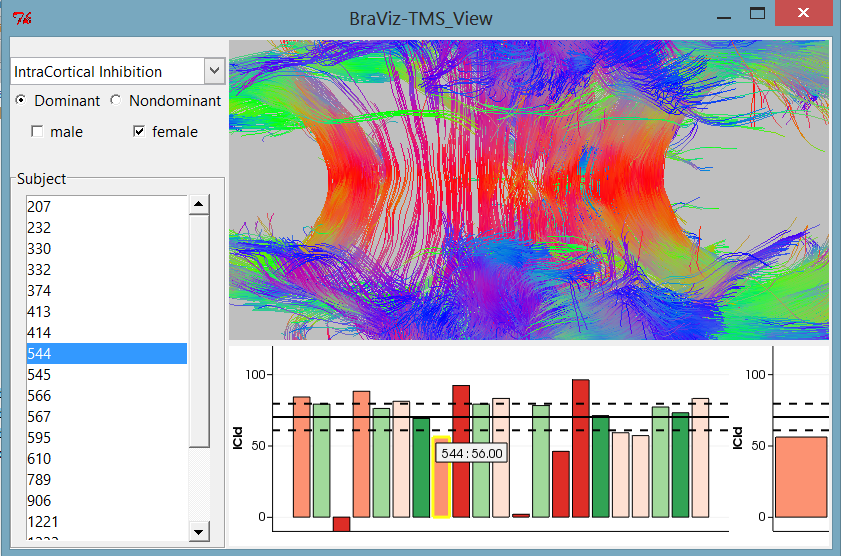
\includegraphics[width=0.90\textwidth]{figures/analysis/tms_view_early}
	\caption{An early version of the TMS viewer application.}
	\label{fig_tms_view_early}
\end{figure}

Figure \ref{fig_tms_view_early} shows an earlier version of the application. In the top left side it had a combo-box for selecting one of the different outcomes. The radio buttons below allowed the researcher to choose between the metrics for the dominant or non-dominant side. Finally there was a list of subjects which could be filtered to show only males, only females or both. At the top right there was a 3D viewer which would display a relevant fiber bundle related to the current outcome. Specifically for intra-cortical measures it would show the motor fibers for the corresponding hemisphere (as in figure \ref{fig_tms_1}) while the corpus callosum would appear for Inter-hemispheric measures.
Below there was a bar plot showing the values of the current outcome for the current subject, together with a large display of this value on the right. The solid and dotted lines in the plot correspond to the mean and the interval within one standard deviation; these statistics are calculated considering only the subjects in the control group. Bars inside this interval are colored green while those outside are colored in red.
This layout was first designed on paper with one of the group researchers. 

The user could move through subjects either by selecting a code on the list or by clicking on one of the bars. The bar at the right would change to the new value, using a transition to accentuate the difference. The image will also change to that of the new subject. This simple tool allows the researcher to navigate between the TMS-outcomes while looking at the underlying white matter structure. 

\begin{figure}
	\centering
		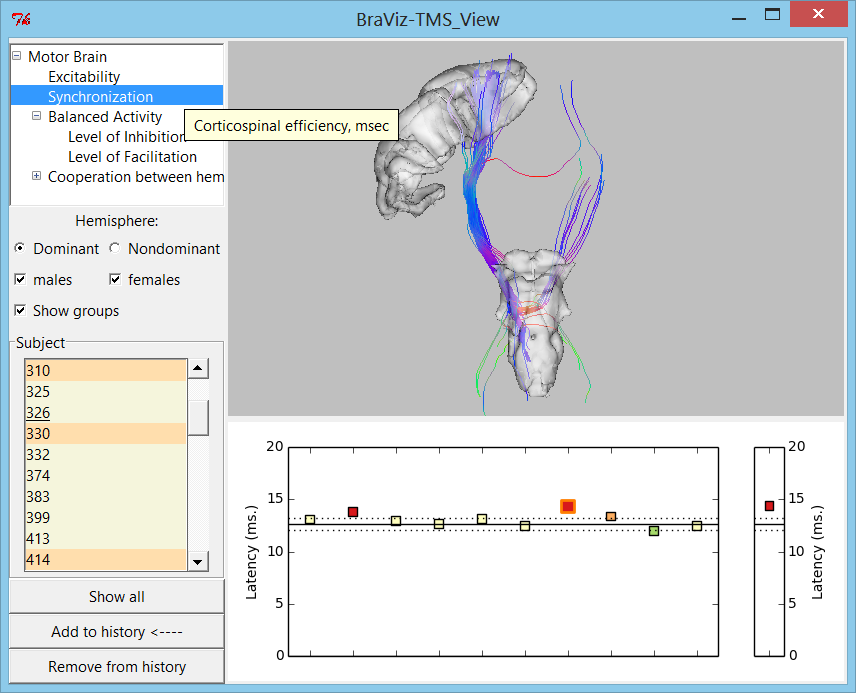
\includegraphics[width=0.90\textwidth]{figures/analysis/tms_view_motor}
	\caption{A second version of the TMS-viewer application}
	\label{fig_tms_view_second}
\end{figure}

Figure \ref{fig_tms_view_second} shows a posterior version of this tool. After receiving feedback from the group, several improvements were made:
\begin{itemize}
	\item TMS outcomes are now organized in a tree, and more descriptive names are used. The purpose is to provide meaning to experts who have limited experience with TMS. Additionally tooltips were added in order to provide additional information on each metric.
	\item The underlying study involved three groups: kangaroo mother care, incubator and control. For some analysis it is convenient to be blind about these groups, but some other times it is beneficial to have this information. Now there is an option to show the different groups in the list of subjects by using different background colors.
	\item The axes in the plot are more clearly labeled and measurement units are shown. 
	\item For some outcomes a higher value is better, while for some others a lower value is better. Now values of the second type are showed using squares instead of bars.
	\item Colors in the main plot were redefined. Now red can be read as \emph{worst than controls}, yellow as \emph{similar to controls} and green as \emph{better than controls}.
	\item The main plot can show the complete sample or only some interesting subjects. The user may add or remove subjects to this sub-sample using the buttons below the subject list.
\end{itemize}

Another round of feedback produced the version shown in figure \ref{fig_tms_2}. This version included additional information in the 3D viewer in order to help users interpret it. The other major feature was showing grouped data in the main plot for the three groups in the study.

This tool allowed experts to .................\footnote{Help Cyril}.


% Veronique Manip
% finding correlations

Another common task found in several of the current experiments was finding correlations between dependent variables. This process was usually done by testing each pair of variables independently. \emph{Aabel} provides a correlation matrix, which is a nice improvement, but it is possible to go further. In a group with several young researchers\footnote{Vero, Hugo, LD} an application for testing correlations was designed. The result of this effort is the \emph{CorrelationsViewer} application shown in figure \ref{fig_correlations}. It is included in the Braviz set, but can also be used as a stand-alone application (available at \url{https://github.com/diego0020/correlation_viewer}). In the stand-alone version the application loads data from an excel file where each row is a subject and each column a variable. The tool interface is divided in three. The first component is a list of variables, each of them with a check-box; it is used to add or remove variables from the analysis. Next is a correlation matrix which encodes in colors the degree of correlation between each pair of variables. Finally, when the user clicks on a square of the matrix the corresponding scatter plot is shown together with the $r$ and $p$ values from the Pearson correlation. An important feature is that individual points can be removed from analysis by clicking on them in the scatter plot. This feature was added because extreme cases can give the impression of a high correlation, however this effect can disappear when the case is removed. The application was refined through several feedback sessions in the group, and several bugs were discovered and corrected.  Below is a testimony from one of the researchers.

\begin{quote}
During the last year, I had the chance to test the new computer program named CorrelationViewer. This program allows visualizing correlations between multiple series of variables. For instance, in my last study, I tested several outcomes that improved after a treatment. I used CorrelationViewer to determine whether my outcomes changes could be related to each other. An interesting feature is the colour scale allowing a quick recognition of the outcomes related altogether. Indeed, this colour scale (gradient red to gradient blue) informs firstly about the direction of the correlation (positive vs. negative). Also, the possibility to visualize easily each linear regression by clicking directly on the wanted correlation is important and practical. You can look at the correlation distribution and whether few participants drive the relation. Above the graph, the p and r stats allow me to determine rapidly whether this graph is pertinent in my research project. Finally, another interesting feature is the possibility to click on a point in the graph and to exclude it from the relation. In this case, new p and r stats are automatically calculated. It allows spotting and excluding easily potential outliers from the project.

With CorrelationViewer, I spent less time to handle the data from one program to the other and I could detect easily and quickly the outcomes correlated altogether. It is an easy and practical tool to use when I do my stats. 
\end{quote}

The \emph{Anova} and \emph{Linear Model} applications (see figures \ref{fig_anova_2} and \ref{fig_lm_2}) were also inspired but the current research questions and workflows in this team. Commonly they have a treatment variable, confounders, and outcomes. The objective is assessing if the treatment has any effects after controlling for confounders, which is tested using ANOVA or two way ANOVA if before and after data is available. The Braviz applications stream-line this testing by letting users conveniently choose the variables for the analysis (no need to format tables each time), presenting results graphically and allowing deeper exploration of outliers. The application is more efficient when used together with other Braviz applications that generate scalar data. This new data can be used directly in an ANOVA analysis without any need to import or export data, and without dealing with files or file formats.

% Anna Belle Manip
% Hugo Manip
% 
% ANOVA - LM

% Alyssa

A neonatologist\footnote{Alyssa} who worked at the hospital provided her opinion of the system from the clinical point of view. She thought that such a tool would be very useful in order to talk the kid's parents, and better explain any findings. If the sample from the current study showed positive results in a similar case, this evidence could be shared with parents to reassure them. It would be also helpful to have all data from a given subject as well as reference data in order to understand the factors that affect a prognosis. 

%insights from cyril's interview
% Visuals are very important. 

In a follow up interview with the head of the lab, he gave us his impressions about the complete system. First of all he was concerned about how new users could get up to speed. He proposed that the first screen should guide the user. What should he do first? There should be a tutorial, and it should be enough so that the user can beyond intuitively. Additionally, he expressed that the user should never be puzzled by the tool itself. This means that the main format should be consistent. There should not be any surprises. The tool should also provide some guidance on relevant data for specific questions. 

As a possible application, he stated that the tool should help in understanding subjects which are not part of the original sample. Given a new subject, it should help me find similar subjects in the sample. It would be specially useful if there are no images of the new subject but the images of existing subjects with similar characteristics are available. 

He also emphasized that this system should be targeted to multiple users expert in multiple domains. The point was not transforming each user into an expert in everything, but to help experts work together and provide a full picture of each subject. With current technologies data from different domains are out of reach, because tools are not compatible, it's hard to understand, and the links between domains are not evident. This causes subjects to be divided into different dimensions. To counter this it is necessary to use a common language that makes links easier to see. By looking at each subject as a whole the tool humanizes research. In this way Braviz could also be very valuable in teaching. 

The tool should let users be very efficient at their work and never make them waste time. It should also be very accurate, as any mistake would cause experts to loose trust in the tool, and all benefits would be lost. No one would want to use a tool that produces results that must be double checked.

He agreed with the user centered approach, and remarked that tools should for end-users should be designed by those end-users, but engineers would always be required.

A final remark was that \emph{knowledge depends on the hypotheses, and the hypotheses on the technology available for testing the questions raised}. 


%%
%KMC
%	Marin
%	Rejean
%	Nathalie

% Video Conference from Iowa
% D:\dropbox\Dropbox\VaBD\ProyectoSavingBrains\minutas_demos_04_14.odt
% Ste Irenne

% lock patient

\section{Interest Surveys}
%NIDCAP
%Guttman's lab

In order to evaluate the interest of the community for a tool such as Braviz, a survey was administered at the NIDCAP conference at Barcelona on October 26, 2014. The attendants to the conferences were pediatricians and neonatologists from around the world. 

Before applying the survey, Dr Charpak gave a demonstration of the tool. The first part of a question asked participants how much they agreed with a set of statements, using a likert scale. The results from this question can be seen in table \ref{tab_nidcap_likert}. 

\begin{table}
	\centering
		\begin{tabular}{p{0.6\textwidth}ccccc}
			\toprule
			Statement&1&2&3&4&5 \\
			\midrule
			The presented tools (Braviz) would support my line of work. & 5 &-&-& 2 &- \\
			Interactive visualization with access to individual detailed information is a key feature. &7&-&-&-&- \\			
			The possibility to explore images (MRI, DTI, fMRI) in the context of other variables, adds value to the analysis. &7&-&-&-&- \\
			The integration of basic statistical tools to the interactive exploration is a valuable feature &7&-&-&-&- \\
			I would be willing to test these tools using my own data in a near future (months) & 6 &-& 1 &-&- \\
			\bottomrule
		\end{tabular}
	\caption{Answers to the survey applied at NIDCAP, 2014. In the first part of the survey, participants should indicate how much they agreed with the listed statements. The scale was
	1: Totally agree, 2: Agree, 3: Neutral, 4: Disagree and 5: Totally disagree. The table shows the number of participants who answered with each value.}
	\label{tab_nidcap_likert}
\end{table}

The second question was: With what frequency do you make visualizations of your data? The possible answers and the number of participants who selected them were:

\begin{itemize}
	\item It's always the first thing I do : No one
	\item Almost always: four participants
	\item Only when I notice something odd: one participants
	\item Rarely: one participant
	\item Just to publish or socialize results: No one
\end{itemize}

The following questions asked : Which tools, similar to the one presented, do you know of? and how satisfied are you with these tools? The answers were 
\begin{itemize}
	\item Conventional T1, T2, MRI, DWI, FA. Very satisfied.
	\item Computarized order entry ( CPOE ). Very satisfied.
	\item Not a single tool, but several specialized tools: cognitive potentials, tractography, etc. Very satisfied.
\end{itemize}

The rest of participants left this space empty. The next question asked: What additional features would you like to find in a visual exploration tool? Participants wrote the following answers
\begin{itemize}
	\item Templates. Volume of structures and tractography data are best if used to combine with functional data in the follow up activity. 
	\item Vermis volumetric analysis.
	\item New techniques as analysis of electical activity using EEG and Bayley III curves for followup. 
	\item Orthogonal visualization of brains, ordinal variables, anova with nominal and ordinal outcomes, comparison with standard values.
\end{itemize}

This survey was also applied at the Center for Neurological Images at Brigham and Women's hospital in Botson, MA, USA. This activity was conducted on June, 2015. The methodology was also a quick demo followed by the survey. This group is composed of physicians (neurologists and radiologists), biologists and engineers, who work in brain image research. 

\begin{table}
	\centering
		\begin{tabular}{p{0.6\textwidth}ccccc}
			\toprule
			Statement&1&2&3&4&5 \\
			\midrule
			The presented tools (Braviz) would support my line of work. & 1 & 3 &-& - & - \\
			Interactive visualization with access to individual detailed information is a key feature. &4&-&-&-&- \\			
			The possibility to explore images (MRI, DTI, fMRI) in the context of other variables, adds value to the analysis. &4&-&-&-&- \\
			The integration of basic statistical tools to the interactive exploration is a valuable feature &4&-&-&-&- \\
			I would be willing to test these tools using my own data in a near future (months) & 3 & 1 & - &-&- \\
			\bottomrule
		\end{tabular}
	\caption{Answers to the survey applied at BWH, 20145. See table \ref{tab_nidcap_likert}.}
	\label{tab_bwh_likert}
\end{table}

The answers to the following questions were

\begin{itemize}
	\item With what frequency do you make visualizations of your data?
	\begin{itemize}
		\item It's always the first thing I do : one participant
		\item Almost always: two participants
		\item Rarely one participant
	\end{itemize}
	\item Which tools similar to the one presented, do you know of? How satisfied are you with these tools?
	\begin{itemize}
		\item Sear, very satisfied
		\item Spine, very satisfied
	\end{itemize}
	\item What additional features would you  like in a visual exploration tool?
	\begin{itemize}
		\item Interactive feature selection (for example all white matter lesions)
		\item Atlases, multiple statistics module (for both descriptive and analysis), database selection \& matching tools, export results and images, voxel-wise analysis, TBSS.
	\end{itemize}	
\end{itemize}

\smallskip

While the sample is small, the survey shows there are multiple specialists willing to try these tools. Most of the participants consider visualization an essential part of analysis, and find value in integrating spatial and clinical data. On the other hand none of them complained about the tools they currently use. This supports our hypothesis that Braviz will not replace any of these tools but complement them. Additionally the survey shows that there is a large interest in integrating more data types and statistical analyzes. Finally, several of the experts are willing to participate in longer studies, so in the future we will be able to collect more data about how these tools can be used in diverse projects.


\section{Group Test}

In addition to the valuable input received by the team of researchers who were present during the development of the tool, it was important to receive feedback from new users. In consequence, a series of training and analysis sessions were carried out. An additional objective was analyzing how interactive visualizations helped communication among specialists, therefore analysis sessions were conducted in couples. The full report of these experiments can be found as an appendix. 

The methodology used in these experiments was inspired by case based studies, and took into account the advise found in \autocite{lam_seven_2011}. In particular, it was clear that numeric measures were not appropriate for analyzing the proposal. Perer \autocite{perer_integrating_2008} recommends that users should work with their own data and on their own projects; so that they have legitimate motivation to explore the database. Unfortunately this was not possible as it is still hard to find specialists working on data-sets that integrate neuro-images with clinical data at a large scale. For this reason, the KMC data-set was used on the experiment. 

Before coming to the lab, a phone interview was applied to the participants in order to understand their background and interests. This interview also inquired about previous experience with analysis and visualization tools. The participants were radiology interns, physicians, psychologists, neurologists and neuroscience PHD students. During the first part of the activity, the dataset was introduced. Afterwards participants were asked to raise questions or hypotheses based on the data-set and explain how they would proceed to answer them. Afterwards a practical introduction to BRAVIZ was given where users followed along in the assigned computers. Then they were asked to revisit their questions, and write if and how they could proceed using BRAVIZ. Then  they were given time to work on pairs on answering some of the questions. The researchers were available in the room to answer questions and provide guidance. Finally, there was a group-wise discussion on the activity, the findings of each group, and free talk about the proposed software. The whole session was recorded, and software logging was used. 

Participants agreed that having plots and graphics available at all time allowed them to notice errors and problematic data opportunely and therefore save time. They also found useful the tools for exploring outliers and deciding what to do about them. It was also evident that the showing these graphics to a colleague was an effective way of communication. Most users went on to try different variable combinations and different visualizations after finishing with the original question, raising more questions in the process. The most used tools were ANOVA and Linear Models, as most questions involved group comparisons. There was also a clear bias of each person towards variables and tools related to their area of expertise.  Not surprisingly, only radiologists attempted to user regions of interests.  

The experiment also highlighted some issues and limitations of the tools. Several controls were not clear and sometimes the labels used too technical terms which were not obvious for participants from different specialties. There were also problems understanding that samples were set individually on each application, and in moving variables form one application to another. All of these were fixed after the experiment. 

However, the biggest problem was in navigating a foreign data-set. It was clear that the current meta-data is not enough to let a new participants find their way around the data. Most of the issues during the experiment were not being able to find the correct variables. During the second and third iterations of the experiment, there was a large effort to clearly explain the naming conventions in the database and providing additional material (variables catalogs) to help participants find variables, but this was still not enough. Most participants agreed that it would be nice to add features to locate variables using keywords, and to organize variables in a hierarchy. Additionally it would be convenient to let each user select a sub-set of variables for each session instead of having to deal with the whole list all the time. In the future, it should be a priority to address this, in order to increase the potential of sharing a dataset with the world.


\section{Feature Model}

%Consequence of the model

The process used to build applications for the Braviz suite is based on the feature model described in chapter \ref{chap_model}. This model presents the commonalities and variability inside the set of applications. The Braviz library provides a set of reusable components that can be used to streamline the construction of new applications. The model of figure \ref{fig_feature_problem} describes the design space at the problem level. It is independent of an application and is best used to design new applications at a high level. This model should be used in the early stages of application design. 

The model represented in figure \ref{fig_feature_solution} is a low level model, coupled with the current implementation. It should be used after the problem space model in order to define the best option to implement the required set of features. 

\begin{table}
\scriptsize
\begin{tabular}{llllllllllllllll}
\toprule
{} & \rot{RoiBuilder} & \rot{LogicBundles} & \rot{LinearMeasure} & \rot{subjOverview} & \rot{sampleOverview} & \rot{CheckRegistration} & \rot{ExploreFMRI} & \rot{Anova} & \rot{LinearModel} & \rot{Histogram} & \rot{Correlations} & \rot{ParallelCoordinates} & \rot{SubjectSwitcher} & \rot{CalculateFeatures} & \rot{PopulateCache} \\
\midrule
SpatialVis           &       \checkmark &         \checkmark &          \checkmark &         \checkmark &           \checkmark &              \checkmark &        \checkmark &             &                   &                 &                    &                           &                       &                         &                     \\
Two                  &                  &                    &                     &                    &                      &                         &                   &             &                   &                 &                    &                           &                       &                         &                     \\
Three                &       \checkmark &         \checkmark &          \checkmark &         \checkmark &           \checkmark &              \checkmark &        \checkmark &             &                   &                 &                    &                           &                       &                         &                     \\
Images               &       \checkmark &         \checkmark &          \checkmark &         \checkmark &           \checkmark &              \checkmark &        \checkmark &             &                   &                 &                    &                           &                       &                         &                     \\
Surfaces             &       \checkmark &         \checkmark &                     &         \checkmark &           \checkmark &                         &        \checkmark &             &                   &                 &                    &                           &                       &                         &                     \\
Tractography         &       \checkmark &         \checkmark &                     &         \checkmark &           \checkmark &                         &                   &             &                   &                 &                    &                           &                       &                         &                     \\
Segmentation         &                  &                    &                     &         \checkmark &           \checkmark &                         &                   &             &                   &                 &                    &                           &                       &                         &                     \\
NonSpatialVis        &                  &                    &                     &                    &           \checkmark &                         &        \checkmark &  \checkmark &        \checkmark &      \checkmark &         \checkmark &                \checkmark &                       &                         &                     \\
Bars                 &                  &                    &                     &                    &           \checkmark &                         &                   &             &                   &                 &                    &                           &                       &                         &                     \\
Scatter              &                  &                    &                     &                    &                      &                         &                   &  \checkmark &        \checkmark &                 &         \checkmark &                           &                       &                         &                     \\
Histogram            &                  &                    &                     &                    &                      &                         &                   &             &                   &      \checkmark &                    &                           &                       &                         &                     \\
BoxPlot              &                  &                    &                     &                    &                      &                         &                   &  \checkmark &                   &                 &                    &                           &                       &                         &                     \\
Spider               &                  &                    &                     &                    &                      &                         &                   &             &                   &                 &                    &                           &                       &                         &                     \\
TimeLine             &                  &                    &                     &                    &                      &                         &        \checkmark &             &                   &                 &                    &                           &                       &                         &                     \\
ParallelCoordinates  &                  &                    &                     &                    &                      &                         &                   &             &                   &                 &                    &                \checkmark &                       &                         &                     \\
SaveRestore          &       \checkmark &         \checkmark &          \checkmark &         \checkmark &           \checkmark &                         &        \checkmark &  \checkmark &        \checkmark &                 &                    &                           &                       &                         &                     \\
Log                  &       \checkmark &         \checkmark &          \checkmark &         \checkmark &           \checkmark &                         &        \checkmark &  \checkmark &        \checkmark &                 &                    &                \checkmark &                       &                         &                     \\
SendSample           &                  &                    &                     &         \checkmark &           \checkmark &                         &        \checkmark &  \checkmark &        \checkmark &                 &         \checkmark &                \checkmark &            \checkmark &                         &                     \\
SendSubject          &                  &                    &                     &         \checkmark &           \checkmark &                         &        \checkmark &  \checkmark &        \checkmark &                 &         \checkmark &                \checkmark &            \checkmark &                         &                     \\
SendVisualization    &                  &                    &                     &         \checkmark &                      &                         &                   &             &                   &                 &                    &                           &                       &                         &                     \\
SendVariables        &                  &                    &                     &                    &                      &                         &                   &  \checkmark &        \checkmark &                 &                    &                           &                       &                         &                     \\
ReceiveSample        &                  &                    &                     &         \checkmark &           \checkmark &                         &        \checkmark &  \checkmark &        \checkmark &      \checkmark &         \checkmark &                \checkmark &            \checkmark &                         &                     \\
ReceiveSubject       &                  &                    &                     &         \checkmark &           \checkmark &                         &        \checkmark &  \checkmark &        \checkmark &      \checkmark &         \checkmark &                \checkmark &            \checkmark &                         &                     \\
ReceiveVisualization &                  &                    &                     &                    &           \checkmark &                         &                   &             &                   &                 &                    &                           &                       &                         &                     \\
ReceiveVariables     &                  &                    &                     &                    &                      &                         &                   &             &                   &                 &         \checkmark &                \checkmark &                       &                         &                     \\
Graphical            &       \checkmark &         \checkmark &          \checkmark &         \checkmark &           \checkmark &              \checkmark &        \checkmark &  \checkmark &        \checkmark &      \checkmark &         \checkmark &                \checkmark &            \checkmark &                         &                     \\
CommandLine          &                  &                    &                     &                    &                      &                         &                   &             &                   &                 &                    &                           &                       &              \checkmark &          \checkmark \\
DefineRegions        &       \checkmark &                    &                     &                    &                      &                         &                   &             &                   &                 &                    &                           &                       &                         &                     \\
ManualMeasure        &                  &                    &          \checkmark &                    &                      &                         &                   &             &                   &                 &                    &                           &                       &                         &                     \\
ManualSegmentation   &                  &                    &                     &                    &                      &                         &                   &             &                   &                 &                    &                           &                       &                         &                     \\
Filter               &       \checkmark &         \checkmark &                     &         \checkmark &           \checkmark &                         &        \checkmark &             &                   &                 &                    &                           &                       &              \checkmark &          \checkmark \\
Isosurfaces          &                  &                    &                     &         \checkmark &           \checkmark &                         &        \checkmark &             &                   &                 &                    &                           &                       &              \checkmark &          \checkmark \\
Transform            &                  &         \checkmark &          \checkmark &         \checkmark &           \checkmark &              \checkmark &        \checkmark &             &                   &                 &                    &                           &                       &              \checkmark &          \checkmark \\
LinearModels         &                  &                    &                     &                    &                      &                         &                   &  \checkmark &        \checkmark &                 &         \checkmark &                           &                       &                         &                     \\
Classification       &                  &                    &                     &                    &                      &                         &                   &             &                   &                 &                    &                           &                       &                         &                     \\
Clustering           &                  &                    &                     &                    &                      &                         &                   &             &                   &                 &                    &                           &                       &                         &                     \\
NonParametric        &                  &                    &                     &                    &                      &                         &                   &             &                   &                 &                    &                           &                       &                         &                     \\
\bottomrule
\end{tabular}
	
\caption{\label{tab_features_problem} Configurations of the current applications in relation to the problem space feature model( see figure \ref{fig_feature_problem}).}
\end{table}

Table \ref{tab_features_problem} shows the features from the problem space model used in the applications available in the current version. Applications are sorted from left to right based on their categories. First are the applications that allow users to generate new data based on images, followed by the applications designed to explore spatial data, then those designed to explore tabular data and perform statistical analyzes and finally some command line utilities that can be used to prepare data for analysis. Some of the features are not yet used in any applications, but they will probably be needed in future developments. Specifically there is evidence of the need to integrate more advanced statistical and machine learning functions to aid in the analysis. 

\begin{table}
\scriptsize
\begin{tabular}{llllllllllllllll}
\toprule
{} & \rot{RoiBuilder} & \rot{LogicBundles} & \rot{LinearMeasure} & \rot{subjOverview} & \rot{sampleOverview} & \rot{ExploreFMRI} & \rot{CheckRegistration} & \rot{Anova} & \rot{LinearModel} & \rot{Correlations} & \rot{Histogram} & \rot{ParallelCoordinates} & \rot{SubjectSwitcher} & \rot{CalculateFeatures} & \rot{PopulateCache} \\
\midrule
CommandLine          &                  &                    &                     &                    &                      &                   &                         &             &                   &                    &                 &                           &                       &              \checkmark &          \checkmark \\
Web                  &                  &                    &                     &                    &                      &                   &                         &             &                   &                    &      \checkmark &                \checkmark &            \checkmark &                         &                     \\
D3                   &                  &                    &                     &                    &                      &                   &                         &             &                   &                    &      \checkmark &                \checkmark &                       &                         &                     \\
Bootstrap            &                  &                    &                     &                    &                      &                   &                         &             &                   &                    &                 &                \checkmark &            \checkmark &                         &                     \\
three                &                  &                    &                     &                    &                      &                   &                         &             &                   &                    &                 &                           &                       &                         &                     \\
DesktopGUI           &       \checkmark &         \checkmark &          \checkmark &         \checkmark &           \checkmark &        \checkmark &              \checkmark &  \checkmark &        \checkmark &         \checkmark &                 &                           &                       &                         &                     \\
MatplotLib           &                  &                    &                     &                    &           \checkmark &        \checkmark &                         &  \checkmark &        \checkmark &         \checkmark &                 &                           &                       &                         &                     \\
VTK                  &       \checkmark &         \checkmark &          \checkmark &         \checkmark &           \checkmark &        \checkmark &              \checkmark &             &                   &                    &                 &                           &                       &                         &                     \\
QtModels             &       \checkmark &         \checkmark &                     &         \checkmark &                      &        \checkmark &                         &  \checkmark &        \checkmark &         \checkmark &                 &                           &                       &                         &                     \\
ReusableQtComponents &       \checkmark &         \checkmark &          \checkmark &         \checkmark &           \checkmark &        \checkmark &              \checkmark &  \checkmark &        \checkmark &         \checkmark &                 &                           &                       &                         &                     \\
SampleManager        &       \checkmark &         \checkmark &          \checkmark &         \checkmark &           \checkmark &        \checkmark &                         &  \checkmark &        \checkmark &         \checkmark &                 &                           &                       &                         &                     \\
ImageManager         &       \checkmark &         \checkmark &          \checkmark &         \checkmark &           \checkmark &        \checkmark &              \checkmark &             &                   &                    &                 &                           &                       &                         &                     \\
ContextPanel         &                  &                    &                     &         \checkmark &                      &                   &                         &             &                   &                    &                 &                           &                       &                         &                     \\
VariableSelectDialog &                  &                    &                     &         \checkmark &           \checkmark &        \checkmark &                         &  \checkmark &        \checkmark &                    &                 &                           &                       &                         &                     \\
Variables            &       \checkmark &                    &          \checkmark &         \checkmark &           \checkmark &        \checkmark &                         &  \checkmark &        \checkmark &         \checkmark &      \checkmark &                \checkmark &                       &                         &                     \\
Samples              &       \checkmark &         \checkmark &          \checkmark &         \checkmark &           \checkmark &        \checkmark &                         &  \checkmark &        \checkmark &         \checkmark &      \checkmark &                \checkmark &            \checkmark &                         &                     \\
Annotations          &                  &                    &                     &         \checkmark &                      &                   &                         &             &                   &                    &                 &                           &                       &                         &                     \\
Images               &       \checkmark &         \checkmark &          \checkmark &         \checkmark &           \checkmark &        \checkmark &              \checkmark &             &                   &                    &                 &                           &                       &              \checkmark &          \checkmark \\
PolyData             &       \checkmark &         \checkmark &          \checkmark &         \checkmark &           \checkmark &        \checkmark &                         &             &                   &                    &                 &                           &                       &              \checkmark &          \checkmark \\
Segmentations        &                  &         \checkmark &          \checkmark &         \checkmark &           \checkmark &                   &                         &             &                   &                    &                 &                           &                       &              \checkmark &          \checkmark \\
Tractography         &       \checkmark &         \checkmark &          \checkmark &         \checkmark &           \checkmark &                   &                         &             &                   &                    &                 &                           &                       &              \checkmark &          \checkmark \\
Surfaces             &       \checkmark &         \checkmark &          \checkmark &         \checkmark &           \checkmark &                   &                         &             &                   &                    &                 &                           &                       &              \checkmark &          \checkmark \\
Contours             &                  &                    &          \checkmark &         \checkmark &           \checkmark &        \checkmark &                         &             &                   &                    &                 &                           &                       &              \checkmark &          \checkmark \\
VTKFilters           &       \checkmark &         \checkmark &                     &         \checkmark &                      &        \checkmark &                         &             &                   &                    &                 &                           &                       &              \checkmark &                     \\
ScipyNumpy           &                  &                    &                     &                    &                      &                   &                         &             &                   &                    &                 &                           &                       &                         &                     \\
R                    &                  &                    &                     &                    &                      &                   &                         &  \checkmark &        \checkmark &         \checkmark &                 &                           &                       &                         &                     \\
Scipy                &                  &                    &                     &                    &                      &                   &                         &             &                   &         \checkmark &                 &                           &                       &                         &                     \\
SphericalRoi         &       \checkmark &                    &                     &                    &                      &                   &                         &             &                   &                    &                 &                           &                       &                         &                     \\
LinearMeasure        &                  &                    &                     &                    &                      &                   &                         &             &        \checkmark &                    &                 &                           &                       &                         &                     \\
ManualSegmentation   &                  &                    &                     &                    &                      &                   &                         &             &                   &                    &                 &                           &                       &                         &                     \\
SaveRestore          &       \checkmark &         \checkmark &          \checkmark &         \checkmark &           \checkmark &        \checkmark &                         &  \checkmark &        \checkmark &         \checkmark &      \checkmark &                \checkmark &                       &                         &                     \\
Communications       &       \checkmark &         \checkmark &          \checkmark &         \checkmark &           \checkmark &        \checkmark &                         &  \checkmark &        \checkmark &         \checkmark &      \checkmark &                \checkmark &            \checkmark &                         &                     \\
Logging              &       \checkmark &         \checkmark &          \checkmark &         \checkmark &           \checkmark &        \checkmark &                         &  \checkmark &        \checkmark &         \checkmark &      \checkmark &                \checkmark &                       &                         &                     \\
\bottomrule
\end{tabular}
	
\caption{ \label{tab_features_solution} Configurations of the current applications in the solution space feature model( see figure \ref{fig_feature_solution}).}
\end{table}


Moving to the solution space model, the set of features used in each applications looks as shown in table \ref{tab_features_problem}. The order of applications is the same. It can be seen that there is still a large room to explore the design space of web based interfaces. All applications are encouraged to implement workflow features so that they can play nicely with the rest of the system, and the table shows this has been the case. It can also be seen that most applications are able to deal with custom samples, which permits analyzes targeted at a certain group.

Configuring each application based on these models forces the designer to explicitly think about which features should be on each application and take structural decisions before starting to code. The models are implemented in feature IDE \autocite{thum_featureide:_2014}. This package provides a tool for selecting and validating new configurations. By conforming to the model, and making use of the common components provided by the library, it is possible to build new applications targeted at specific analysis tasks that can be integrated into the whole system.

%Show how the model is instantiated on each application

%Planned applications

%Reusable components
%Process, stages
%metrics: time, lines of code
%Other developers: David, Yoyis

\section{Discussion}

% user centered design
Visual analytics tools permit different ways of working with the data. They provide more freedom to users and let them follow their instinct and curiosity to efficiently explore different paths. In order to achieve efficiency tools need to adapt to users. They should be designed to fit into their workflow and environment, and they should use language and interactions that are natural to them. In order achieve this goal end users should be involved in the design and implementation process at all time. The user centered design methodology used in Braviz development allowed it to become a tool that adapts to the need of researchers. This chapter showed how user feedback was considered at every stage. Each time it provided valuable input about missing features, inadequate language or interactions, and opportunities to add new functionality. It is clear that collaboration from domain experts is mandatory for a project such as this one to succeed.

%Visualization benefits
An objective of the platform was providing access to rich visualizations of data on demand. This was meant to let users know all the time where data came from and to investigate anomalies. This has allowed researchers to quickly find errors in data and correct them, and to find interesting subjects which deserve a closer look. With traditional tools such cases could have gone undetected. Nevertheless, several researchers are used to working with data tables and are very proficient at reading them. These users prefer using the data representation they know rather than learning new representations. The proposed system is designed to work well with external tools. Data can be easily exported and imported, which can allow these users to integrate the tool into their current workflow and therefore get the benefits from both worlds.

%Interdisciplinary work
The project was conceived as a tool where researchers from multiple specialties could meet and work together. Up to know it has been successful in bringing experts from the neuro-images community closer to pediatricians, psychologists and economists. In this way each member of the team is able to make a better use of each others work. Communication is also more efficient as everybody has access to the whole data and therefore can match words with visualizations. However the team tends to develop their own language and conventions, for example for naming variables. This creates a barrier for researchers from outside the team when they which to access the data. 

%Need for a long term study
This chapter provides evidence of the need and usefulness of visual analytics in brain data research. However the true benefits of such tools will only be seen in the long term. It is expected that this kind of tools will become standard in large brain research projects. The need for such tools will be more relevant as the size of available data grows and as research teams become more interdisciplinary and distributed.  

%Model and architecture
The architecture and model presented provide a robust and flexible framework that can be used to generate tools tailored at different analysis tasks. By using the components from the common library developers can focus on meeting the user needs. Therefore time and energy is concentrated on providing the best tool for the analysis task instead of solving technical details. Technical challenges will also arise when new applications are conceived, but these challenges should be solved in such a way that they can be reused. Nevertheless the current model provides room for a wide range of applications that can adapt to different situations. Designing new applications using the model ensures that they will integrate well with the rest of the system. An integrated set of applications provides several times more  possibilities to explore data and find interesting patterns and features. 

%What features are the most useful?
%What is feasible now that wasn't at the start?
%What features are missing?
%What limitations have come to light?

%Can these techniques be used on other domains?
The techniques illustrated by this project are not specific to research in brain images. Feature models are a main component of software product lines, a technique that aims to produce software specific for each application while relying on a common set of reusable assets. User centered design is also a recognized technique for building applications that adapt to users. Visual analytics principles can also be applied to every area that has to explore large sets of data looking for the unknown. Therefore there exist several opportunities to apply these techniques to other domains in order to produce sets of integrated applications that can help group of experts increase their comprehension of the data and the underlying systems. The key for success in all these domains will be a conscious effort to involve users, and to analyze the challenges and needs of the domain. 
